\documentclass[
	openboth, % Capítulos começam em página direita
	oneside,   % Impressão frente e verso
	a4paper,   % Tamanho do papel
	english,   % Idioma adiciona para hifenizaçãoo
	brazil     % O ultimo é o idioma principal
]{abntex2}

\usepackage{lmodern}                               % Usa família de fontes Latin Modern
\usepackage[T1]{fontenc}                           % Codifição Type1 para a fonte (Fontes de 8 bits para incluir as fontes do alfabeto brasileiro)
\usepackage[UTF8]{inputenc}                        % Codificação unicode "UTF8"
\usepackage{microtype}                             % Melhorias na justificação (Evita bad/underfullbox)
\usepackage{indentfirst}                           % Indenta o primeiro parágrafo da seção
\usepackage{amssymb}                               % Símbolos matemáticos
\usepackage{enumitem}                              % Melhoria no suporte aos ambientes de numeração
\usepackage{color}                                 % Suporte a cores
\definecolor{blue}{RGB}{41,5,195}                  % Alterando o aspécto da cor Azul
\usepackage{graphicx}                              % Suporte a gráficos e figuras
\usepackage[alf]{abntex2cite}                      % Citações no padrão ABNT

% informações do PDF
\makeatletter
\hypersetup{
	%pagebackref=true,
	pdftitle={\@title}, 
	pdfauthor={\@author},
	pdfsubject={\imprimirpreambulo},
	pdfcreator={LaTeX with abnTeX2},
	pdfkeywords={abnt}{latex}{abntex}{abntex2}{trabalho acadêmico}, 
	colorlinks=true,       		% false: boxed links; true: colored links
	linkcolor=black,          	% color of internal links
	citecolor=black,        		% color of links to bibliography
	filecolor=black,      		% color of file links
	urlcolor=black,
	bookmarksdepth=4
}
\makeatother

% O tamanho do parágrafo é dado por:
\setlength{\parindent}{1.3cm}

% Controle do espaçamento entre um parágrafo e outro:
\setlength{\parskip}{0.2cm}  % tente também \onelineskip





\makeindex
\makeglossary


\AtBeginDocument{
	\pagenumbering{gobble}
	\frenchspacing 
	\pretextual
	\tableofcontents*
	\textual
}

\begin{document}
	\chapter{Introdução}
	\pagenumbering{arabic}
	\setcounter{page}{1}
	
	As preocupações devido às emissões de CO2 tornaram a utilização de fontes de energias renováveis interessantes. Dentre elas, a energia baseada no vento se mostrou bastante promissora, pois o Brasil tem um dos maiores potenciais eólicos do mundo \cite{atlaseolico}.
	
	Com o aumento da participação da matriz eólica surgem novos desafios. A velocidade do vento é uma grandeza com grande variação instantânea, podendo variar bastante em questão de horas ou, até mesmo minutos. Essa variação, se não for contornada, pode trazer problemas de qualidade de energia, como a variação da frequência da rede devido a variação do vento, principalmente em redes mais fracas e dependentes da energia eólica. Além disso, há a presença de harmônicos devido ao movimento caótico do vento e ao efeito de sombra, ou seja, a perda de potência no momento em que uma das pás passa pela torre \cite{pintofundamentos}.
	
	Uma das soluções para melhorar a qualidade de energia de fontes eólicas é uso da eletrônica de potência em conjunto com topologias alternativas de geradores, como o GIDA (Gerador de indução duplamente alimentado).  A escolha do GIDA ocorre devido ao seu conversor processar até 30\% da potência nominal do gerador, enquanto em outros geradores com conversor acoplado esse valor chega a 100\%. Isto possibilita a redução do custo do conversor
	
	\begin{figure}[h]
		\centering
		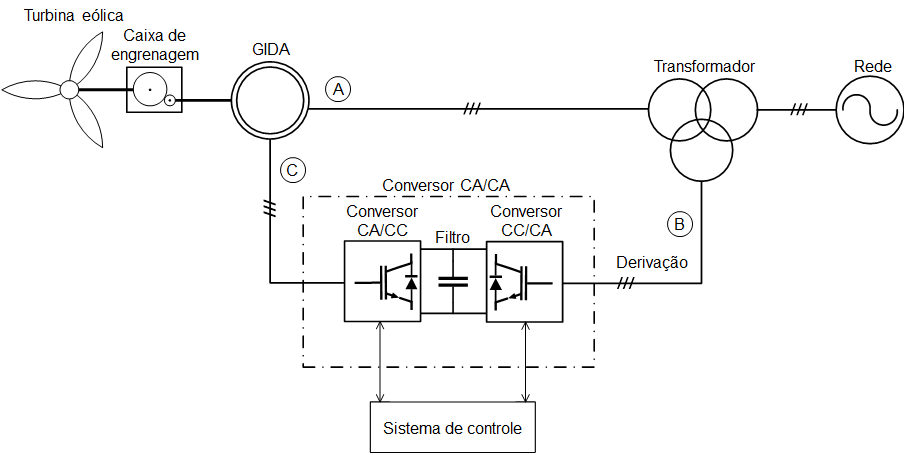
\includegraphics[width=1\textwidth]{Figuras/gida_esquematico.png}
		\caption{Esquema do GIDA conectado à  rede para geração de energia eólica (Próprio autor)}
		\label{figura:gida_esquematico}
	\end{figure}
	
	\bibliographystyle{abntex2-alf}
	\bibliography{biblio}
\end{document}